%%% Simulering for optimering af reguleringsloop %%%

\subsection{Gain-fase}
Simuleringen af systemets gain-fase karakteristik, udføres på samme måde som ved 2. iteration. Bode plot for fejlforstærkeren er vist på figur~\ref{fig:Simulering_error_op_amp_3}. Da knækfrekvensen for fejlforstærkeren ligger ved $132\hertz$, og der ikke kan simuleres med frekvenser lavere end $100\hertz$, er det svært at aflæse bode plottet. Det kan dog aflæses, at forstærkningen over $132^\circ$ ligger sig på ca. $8.6\decibel$. Derudover ses det at fasen stiger til $180^\circ$, derfor antages det, at fejlforstærkeren vil bidrage med det forventede faseløft på $90^\circ$. 

\begin{figure}[H]
	\center
	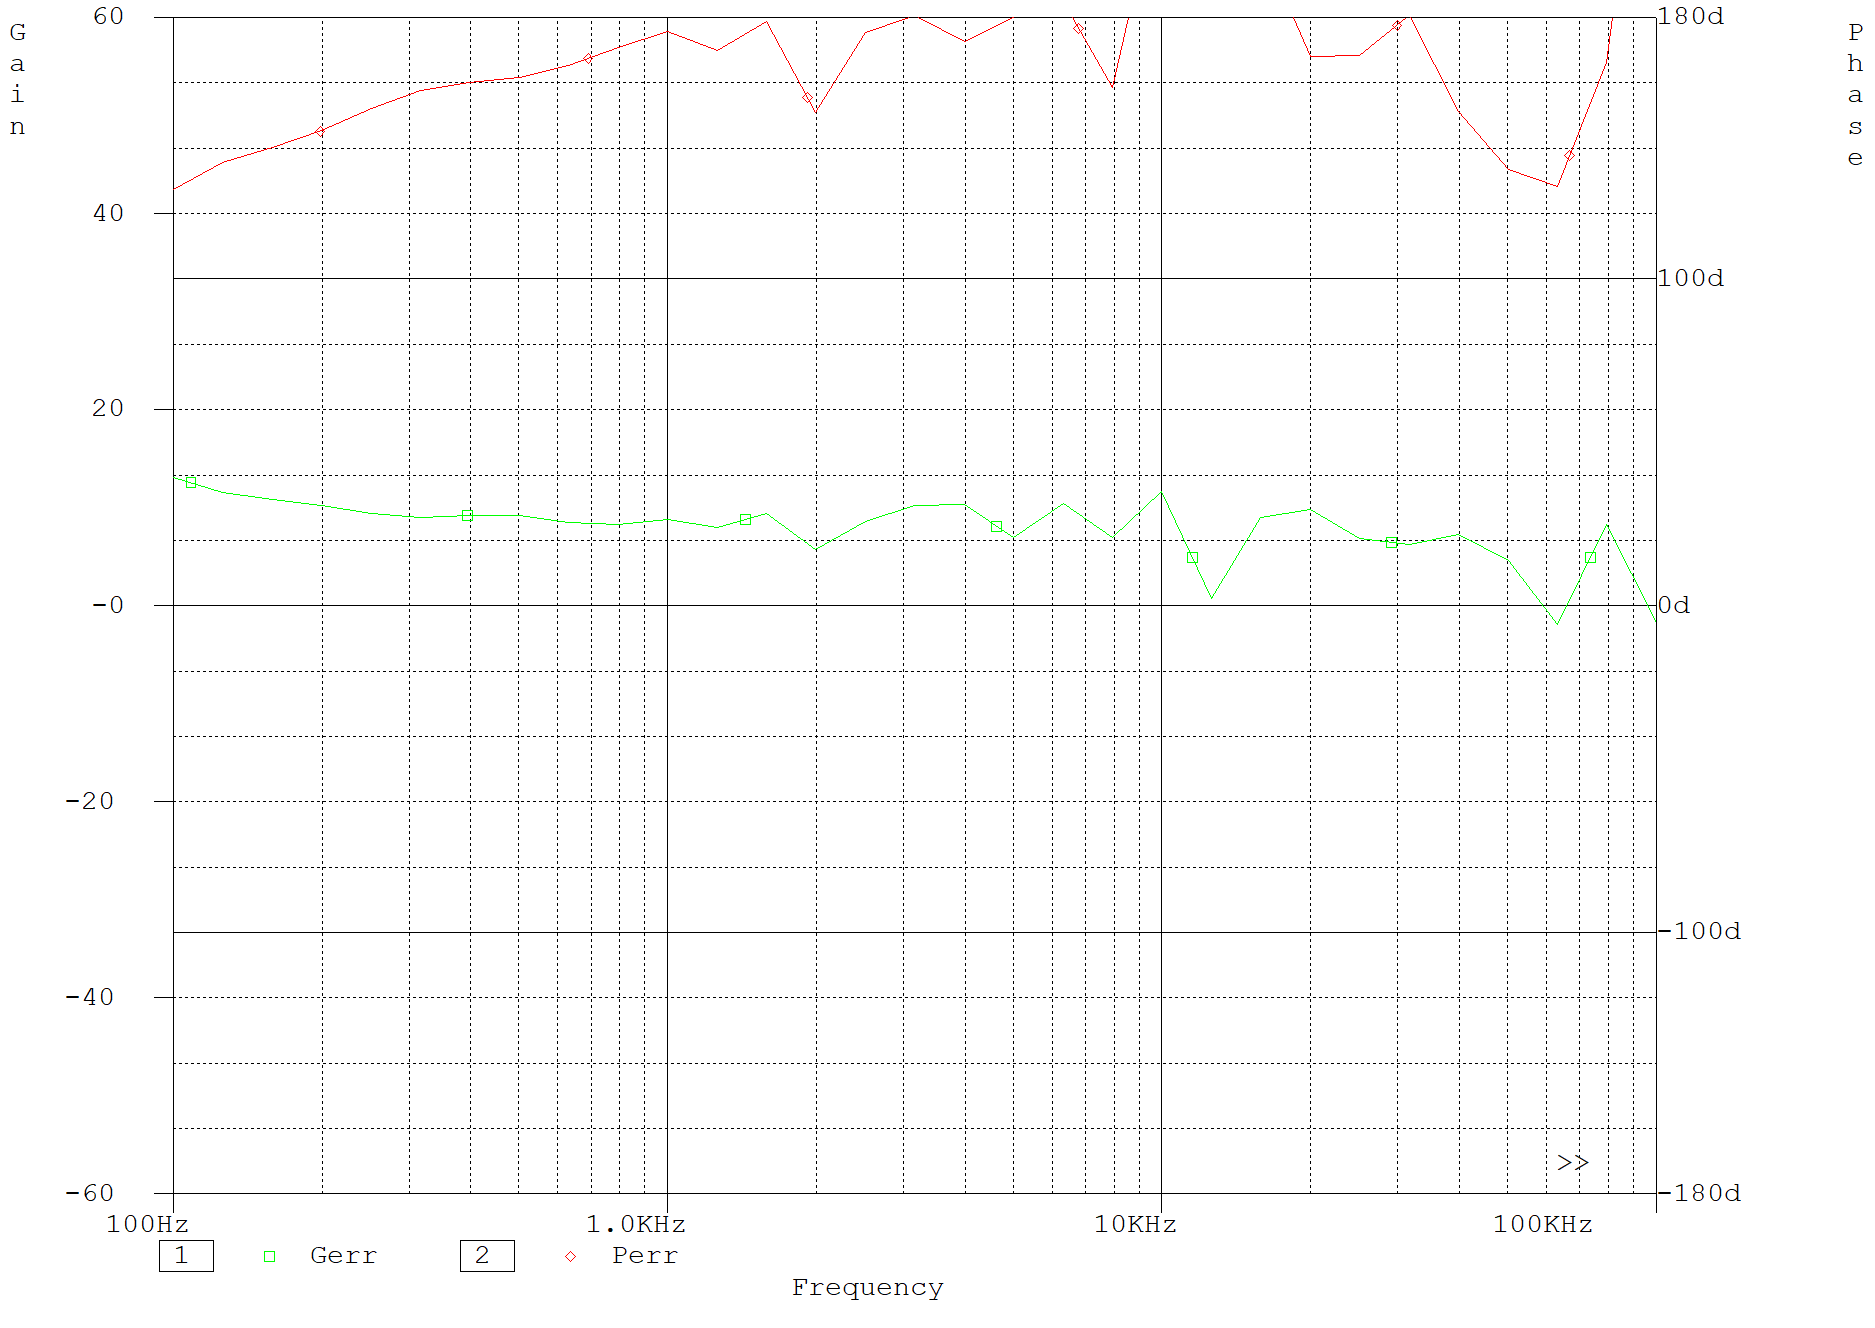
\includegraphics[max width=0.7\linewidth]{/tex/3iteration/billeder/Simulering/Simulering_error_op_amp.PNG}
	\caption{Simulering af fejlforstærkeren}
	\label{fig:Simulering_error_op_amp_3}
\end{figure}

\noindent Bode plottet for det samlede system er vist på figur~\ref{fig:Simulering_total_3}. Selvom simuleringen bliver usikker ved høje frekvenser, sker det så langt oppe i frekvens, at de relevante værdier akkurat kan aflæses. Gain-margin aflæses til ca. $10.2\decibel$, fase-margin aflæses til ca. $73.2^\circ$, og båndbredden aflæses til ca. $3.5k\hertz$. Ift. analysen passer både gain- og fasemargin, mens båndbredden ca. $400\hertz$ lavere end det forventede. 

\begin{figure}[H]
	\center
	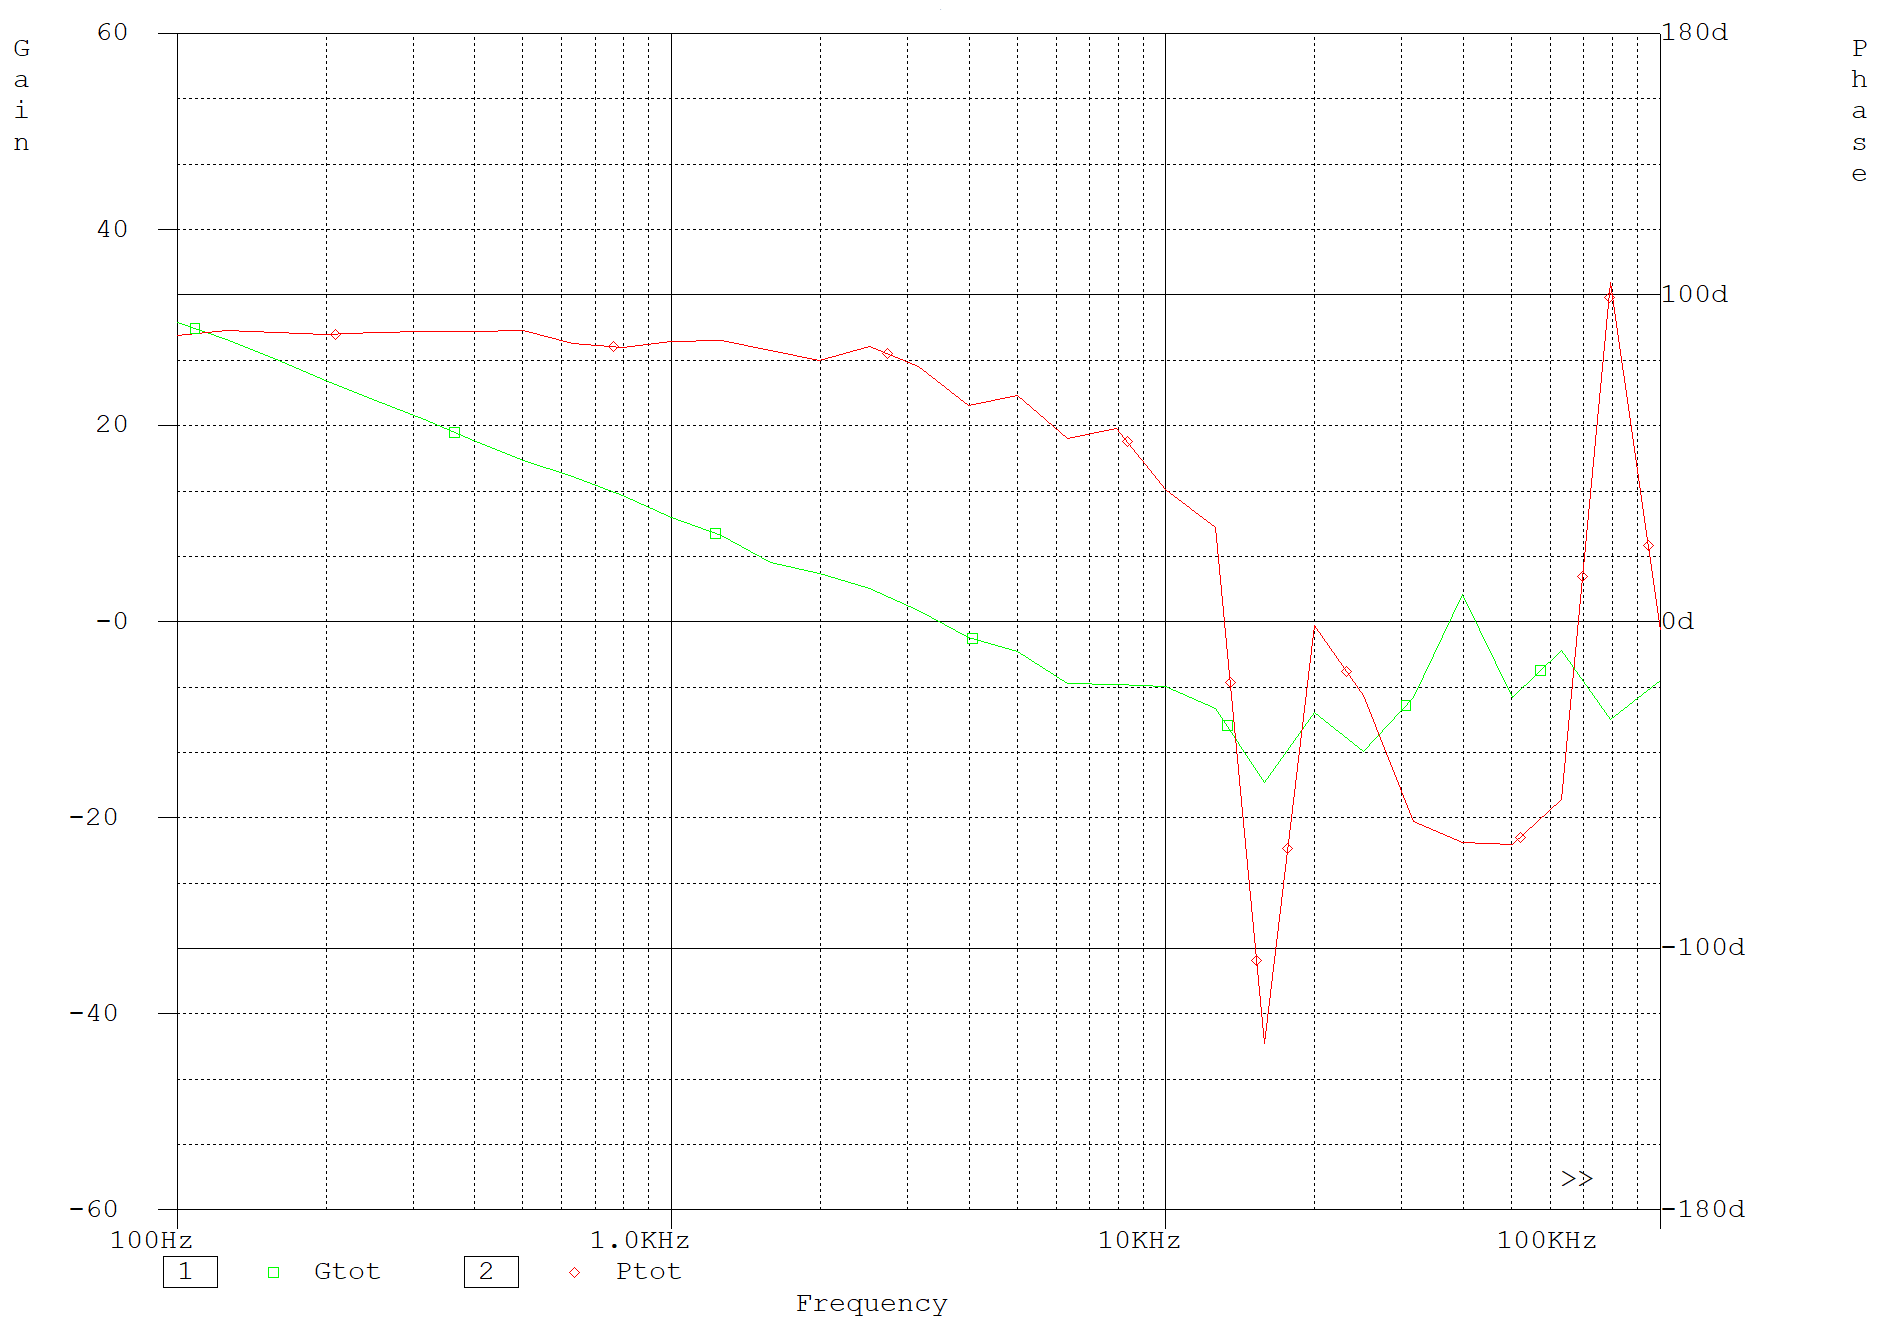
\includegraphics[max width=0.7\linewidth]{/tex/3iteration/billeder/Simulering/Simulering_total.PNG}
	\caption{Simulering af det samlede system}
	\label{fig:Simulering_total_3}
\end{figure}